\documentclass[10pt]{article}
\textwidth = 450pt
\headsep = 2pt
\headheight = 1pt
\oddsidemargin = 1pt

\usepackage{changepage}
\usepackage{fancyvrb}
\usepackage{graphicx}
\usepackage{amsmath}
\usepackage{capt-of}
\usepackage{amsfonts}
\usepackage{verbatim}
\usepackage{courier}
\usepackage{float}
\restylefloat{table}

%%%%%%%%%%%%%%%%%%% Code %%%%%%%%%%%%%%%%%%%%%%
\usepackage{color}
\usepackage[table]{xcolor} %adding background color to your tables
\usepackage{listings}% Allows you to present C++ syntax as it looks
\usepackage{listings} %enables inputing code set the settings below
\definecolor{dkgreen}{rgb}{0,0.45,0}
\definecolor{gray}{rgb}{0.2,0.5,0.5}
\definecolor{mauve}{rgb}{0.58,0,0.82}
%\definecolor{purple}{RGB}}{204, 45, 109}
\lstset{ %
language=C, % choose the language of the code
commentstyle=\color{dkgreen},
basicstyle=\footnotesize, % the size of the fonts that are used for the code
numbers=left, % where to put the line-numbers
numberstyle=\footnotesize, % the size of the fonts that are used for the line-numbers
stepnumber=1, % the step between two line-numbers. If it is 1 each line will be numbered
numbersep=5pt, % how far the line-numbers are from the code
backgroundcolor=\color{white}, % choose the background color. You must add \usepackage{color}
showspaces=false, % show spaces adding particular underscores
showstringspaces=false, % underline spaces within strings
showtabs=false, % show tabs within strings adding particular underscores
frame=single, % adds a frame around the code
tabsize=2, % sets default tabsize to 2 spaces
captionpos=b, % sets the caption-position to bottom
breaklines=true, % sets automatic line breaking
breakatwhitespace=false, % sets if automatic breaks should only happen at whitespace
keywordstyle=\color{purple}, % keyword style
numberstyle=\tiny\color{gray}, % the style that is used for the line-numbers
rulecolor=\color{black}, % if not set, the frame-color may be changed on
stringstyle=\color{blue}, % string literal style
escapeinside={\%*}{*)} % if you want to add a comment within your code
}
\DefineVerbatimEnvironment{code}{Verbatim}{fontsize=\small}
\DefineVerbatimEnvironment{example}{Verbatim}{fontsize=\small}
%%%%%%%%%%%%%%%%%%%%%%%%%%%%%%%%%%%%%%%%%%%%%%%%

\begin{document}
\title{Using Kinect to Evaluate Dance Performances\\ Third Year Group Project}
\author{Stylianos Venieris, Marcin Baginski, Theo Pavlakou, Zeping Xue, \\ Yijie Ge \& Hesam Ipakchi  }
\date{\today}
\maketitle
\newpage

\section*{\center Abstract}

\section{Kinect \& NiTE Software Evaluation}
\noindent
To determine a method of evaluating the dance student, the limitations of the camera and the NiTE software must first be evaluated with respect to the criteria addressed below. To do this we use the UserViewer Application that comes as a sample with the NiTE software library with the camera elevated 75cm above the ground, within the 60cm to 180cm range that is suggested by Microsoft for optimal tracking. 

\subsection{Camera Range}
\noindent 
To test for the camera's range, we lay a tape measure on the ground starting from directly below the camera up to 8m away from the camera. We then use two subjects of different heights and body shapes to evaluate the performance of the camera and the software for tracking at different distances. The subject first starts within a few centimetres of the camera and slowly moves backwards until the camera calibrates and starts tracking and continues to do so until the tracking is lost. After this, the subject is required to start from the depths of the room, much further than the range of the camera, and to start walking slowly towards the camera, again taking a record of the following specifications. The results can be shown in Tables \ref{cam_range_180_away} to \ref{cam_range_150_toward}.
\\
\begin{table}[h]
\center
\begin{tabular}{ | l | c |}
\hline
Distance from Camera/cm & Description of Performance \\
\hline
60 & Identification of subject. Tracking. No skeleton.\\
120 & Skeleton fitted\\
410 & Tracking is lost\\
\hline
\end{tabular}
\caption{Subject moving away from camera. Subject height 180cm.}
\label{cam_range_180_away}
\end{table}

\begin{table}[h]
\center
\begin{tabular}{ | l | c |}
\hline
Distance from Camera/cm & Description of Performance \\
\hline
100 & Identification of subject. Tracking. No skeleton.\\
120 & Skeleton fitted\\
410 & Tracking is lost\\
\hline
\end{tabular}
\caption{Subject moving towards camera. Subject height 180cm.}
\label{cam_range_180_toward}
\end{table}

\begin{table}[h]
\center
\begin{tabular}{ | l | c |}
\hline
Distance from Camera/cm & Description of Performance \\
\hline
70 & Identification of subject. Tracking. No skeleton.\\
110 & Skeleton fitted\\
430 & Tracking is lost\\
\hline
\end{tabular}
\caption{Subject moving away camera. Subject height 150cm.}
\label{cam_range_150_away}
\end{table}

\begin{table}[h]
\center
\begin{tabular}{ | l | c |}
\hline
Distance from Camera/cm & Description of Performance \\
\hline
50 & Identification of subject. Tracking. No skeleton.\\
110 & Skeleton fitted\\
430 & Tracking is lost\\
\hline
\end{tabular}
\caption{Subject moving towards camera. Subject height 150cm.}
\label{cam_range_150_toward}
\end{table}

\subsection{Effect of Varying Lighting Conditions}
\subsection{Obstruction in Range}
\subsection{Velocity of Movement}
Another important criterion regarding the performance of both the Kinect camera and the NiTE software package is the accuracy and responsiveness of the skeleton fitting. Our evaluation procedure consists of the recording of a predefined movement which would provide us with the subject's velocity information and would allow us to estimate how accurately the fitted skeleton is able to follow the actual move, by calculating the error between the perceived and the actual movement. In particular, we would record a slower and a faster versions of the same movement and compare the corresponding errors.

The subject's reference movement was determined to be a $180^o$ degrees right arm move starting from a vertical position with the hand facing the ceiling and following an arc. The testing procedure includes the modification of the \texttt{UserViewer} sample program in order to record twice the predefined movement as performed by the subject at high and low speeds. 

By capturing the recorded passage with a Desktop camera at a rate of 24 frames per second(fps), we are able to extract individual frames from the recorded videos. At this point, we define a starting and an ending point of the subject's right arm and select the frames that more accurately correspond to these positions. After following this procedure for both recordings, we end up with 3 frames from the fast and 16 from the slow version. The starting and ending position frames for the slow and the fast versions are shown below on Figure \ref{start_pos}. The substantial deviation between the shoulder-elbow vertex of the skeleton and the arm indicate the important increased error when the subject performs a fast move.

\begin{figure}[h]
\center
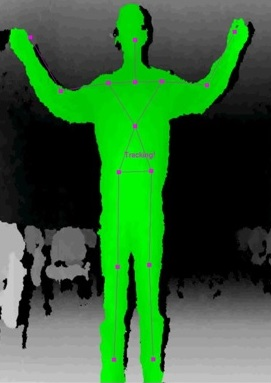
\includegraphics[scale=0.5]{SlowStart.jpg} 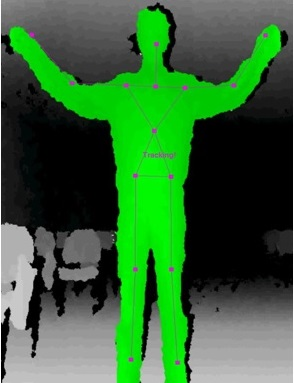
\includegraphics[scale=0.5]{FastStart.jpg}
\caption{Slow and fast recordings starting position.}
\label{start_pos}
\end{figure}

\begin{figure}
\center
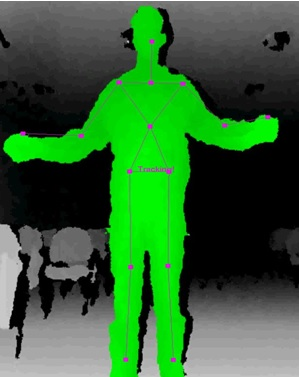
\includegraphics[scale=0.5]{SlowEnd.jpg} 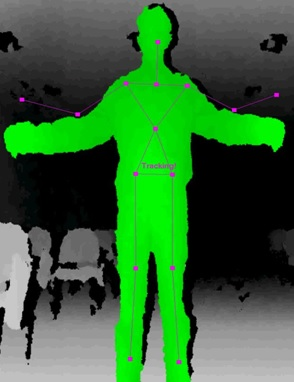
\includegraphics[scale=0.5]{FastEnd.jpg}
\caption{Slow and fast recordings ending position, with substantial error in the fast version's skeleton fitting.}
\end{figure}


\noindent A summary of the number of frames and the time between the starting and ending arm position for each  is shown below.

\begin{table}[H]
\center
\begin{tabular}{| c | c | c |}
\hline
Movement Speed & Number of Frames & Movement Duration/sec\\
\hline
Fast & 3 & 0.083\\
Slow & 16 & 0.670\\
\hline
\end{tabular}
\caption{Movement duration for fast and slow versions, recorded at 24 fps.}
\end{table}

The next step of the responsiveness evaluation is the estimation of the arm's actual starting and ending positions as well as its perceived position as defined by the fitted skeleton. As the arm follows an arc-shaped movement, we focus on measuring the angle between the subject's elbow and shoulder, with the shoulder  defined as the reference, and finding an estimate of the skeleton fitting error by comparing the actual angle and the angle of the vertex between the two joints with respect to the shoulder joint. Although both the actual and perceived starting positions are the same, the ending positions are different and result in errors in the subject's tracking. The angle measurements can be seen below in Table \ref{angle}.

\begin{table}[H]
\center
\begin{tabular}{| c | c | c | c |}
\hline
Movement Speed & Starting Angle/deg & Perceived Ending Angle/deg & Actual Ending Angle/deg\\
\hline
Fast & $3.5^o$ & $-30.5^o$ & $-55.3^o$\\
Slow & $4.4^o$ & $-49.2^o$ & $-64.0^o$\\
\hline
\end{tabular}
\caption{Perceived and actual starting and ending angles of the subject's arm.}
\label{angle}
\end{table}

The final step involved the estimation of the actual and perceived angular velocities based on the already obtained data and the calculation of the error as a consequence to the difference between them. By using the following formula, we estimate the angular velocities and the errors for both the slow and the fast recordings.
\begin{equation}
\omega = RotationalDisplacement * MovementDuration
\end{equation}

\noindent where \[RotationalDisplacement = EndingAngle - StartingAngle\]
and  $\omega$ stands for the angular velocity

\noindent The angular velocities and the corresponding errors for both the slow and the fast recordings are presented on the following table.

\begin{table}[H]
\center
\begin{tabular}{| c | c | c | c |}
\hline
Movement Speed & Perceived Angular Velocity/$^o/s$ & Actual Angular Velocity/$^o/s$ & Error/\% \\
\hline
Fast & $-408.0$ & $-705.0$ & $42.12\%$ \\
Slow & $-67.2$ & $-89.4$ & $24.8\%$ \\
\hline
\end{tabular}
\caption{Perceived and actual angular velocities and percentage errors.}
\end{table}

As a result, ... % CHANGE

\subsection{Camera Angle Relative to Subject}
\subsection{Multiple People}
\subsection{Multiple Cameras}
\clearpage

\section*{Appendix}
\subsection*{Some Code}
\begin{lstlisting}
int main()
{
	// your code
	x = 5;
}

\end{lstlisting}
\end{document}
